\problemname{Heavy Hauling}

\illustration{0.32}{parcel_retriever_robot.jpg}{The Parcel Retriever Robot. \\ CC BY 2.0 by Enrique Dans on Flickr}
% Source: https://www.flickr.com/photos/edans/44492166/in/photostream/

% optionally define variables/limits for this problem
\newcommand{\maxn}{10^6}
\newcommand{\maxx}{10^9}

% Original statement:
% Given $n$ blocks at given positions.
% Moving a block an integer distance $d$ costs $d^2$.
% What is the minimal cost to make all block positions distinct?

The warehouse of the Boxes And Parcels Center (BAPC) just received an official warning from the inspector:
apparently, it does not conform to the latest safety requirements.
In the past, it was allowed to stack multiple boxes at the same shelf location,
but due to the potential fire hazard, this is no longer allowed.
In a hurry, all employees of the BAPC are roused to move the boxes to distinct positions.

After moving the boxes, the automated parcel retriever robot needs to be reprogrammed
such that it knows the correct location of the boxes.
Per box that is moved $d$ positions, it takes $d^2$ time to do this reprogramming.
Of course, the BAPC should be up and running as soon as possible after moving the boxes,
so the boxes should be moved in such a way that this total reprogramming time is as small as possible.
Calculate the minimal time for the reprogramming for an optimal moving of boxes.

The warehouse of the BAPC is unbounded in both directions.

As an example, consider Figure~\ref{fig:heavy-1}, corresponding to the first sample case.
One box at position $-1$ is moved to the left,
which costs $1$ time for the reprogramming.
The box at position $4$ is moved one position to the right,
to make place for one of the boxes at position $3$,
costing $1$ time as well.
Two boxes at position $3$ are moved to the left (costing $1$ and $4$),
and one box at position $3$ is moved to the right (costing $1$),
making the total cost $1+1+1+4+1=8$.

\begin{figure}[h]
    \centering
    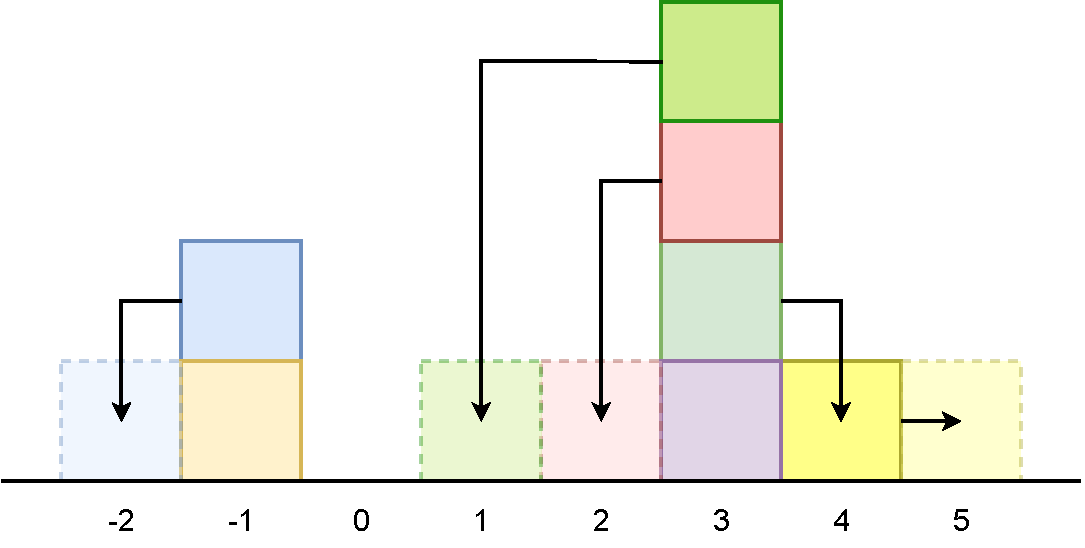
\includegraphics[width=0.45\textwidth]{merged.pdf}
    \caption{Visualisation of the first sample case.}
    \label{fig:heavy-1}
\end{figure}

\begin{Input}
    The input consists of:
    \begin{itemize}
        \item One line with an integer $n$ ($1\leq n\leq \maxn$), the number of boxes.
        \item One line with $n$ integers $x$ ($\left| x \right| \leq \maxx$),
            the position of each box.
            The box positions are ordered non-decreasingly.
    \end{itemize}
\end{Input}

\begin{Output}
    Output the minimal time to reprogram the parcel retriever robot for an optimal moving of boxes.
\end{Output}
